\documentclass[10pt, oneside,english]{article}   	% use "amsart" instead of "article" for AMSLaTeX format
\usepackage{geometry}                		% See geometry.pdf to learn the layout options. There are lots.
\geometry{a4paper}                   		% ... or a4paper or a5paper or ... 
\usepackage[english]{babel}
\selectlanguage{english}
\usepackage[utf8]{inputenc}
\usepackage[font=small,hang]{caption}
\usepackage{hyperref}
\usepackage{adjustbox}
\usepackage[table,xcdraw]{xcolor}
%\geometry{landscape}                		% Activate for rotated page geometry
%\usepackage[parfill]{parskip}    		% Activate to begin paragraphs with an empty line rather than an indent
\usepackage{graphicx}				% Use pdf, png, jpg, or eps§ with pdflatex; use eps in DVI mode
								% TeX will automatically convert eps --> pdf in pdflatex		
\usepackage{amssymb}
\usepackage{authblk}
\usepackage{float}

\usepackage{listings} % for python code

\usepackage{tcolorbox}
\tcbuselibrary{minted,breakable,xparse,skins}

\definecolor{bg}{gray}{0.95}
\DeclareTCBListing{mintedbox}{O{}m!O{}}{%
  breakable=true,
  listing engine=minted,
  listing only,
  minted language=#2,
  minted style=default,
  minted options={%
    linenos,
    gobble=0,
    breaklines=true,
    breakafter=,,
    fontsize=\small,
    numbersep=8pt,
    #1},
  boxsep=0pt,
  left skip=0pt,
  right skip=0pt,
  left=25pt,
  right=0pt,
  top=3pt,
  bottom=3pt,
  arc=5pt,
  leftrule=0pt,
  rightrule=0pt,
  bottomrule=2pt,
  toprule=2pt,
  colback=bg,
  colframe=orange!70,
  enhanced,
  overlay={%
    \begin{tcbclipinterior}
    \fill[orange!20!white] (frame.south west) rectangle ([xshift=20pt]frame.north west);
    \end{tcbclipinterior}},
  #3}
%SetFonts

%SetFonts


\title{Finite State Machine using the Linux kernel interface IO\_URING \\}
\affil[ ]{Francesco Aristei}

						% Activate to display a given date or no date


\begin{document}
    
\maketitle    

\tableofcontents
\newpage

\section{Project Data}

\begin{itemize}
    \item
    Project supervisor: Professor Vittorio Zaccaria
    \item
    Project developer:
    \begin{center}
        \begin{tabular}{lll}
            First and last name & Person code & Email address\\
            \hline
            Francesco Aristei & 10804304 & francesco.aristei@mail.polimi.it \\
        \end{tabular}
    \end{center}

    \item
    Project Repository: Available on \href{https://github.com/francescoaristei/io_uring_fsm}{Github} \\
    I personally worked on the entirety of the repository contents, and wrote all the code and project report myself.

\end{itemize}


\section{Project Description}

A fundamental part of Operating Systems's theory, is represented by how concurrent processes and threads manage to share the processors and the different resources of the system without interfering with each other. \\
The Operating System addresses these issues with several techniques, depending if concurrency happens in user space or kernel space, it can exploit shared memory areas, or through the adoption of shared locks and semaphores.\\
Generally speaking, there are different styles of concurrent programming that can be adopted to solve concurrency problems.\\
It would be interesting to explore some of those, gaining knowledge about less used techniques.\\
One interesting pattern used to address concurrency in user space, is the event-based one.\\
This approach, waits for something (i.e., an “event”) to occur (or “posted” by an external entity) checking what type of event has arrived, identifying which activity it belongs and finally doing the small amount of work it requires.\\
An issue that arises with this kind of model is that if an event handler issues a call that blocks, the entire server will do just that: block until the call completes, wasting resources.\\
Different solutions can be implemented to solve this problem. \\
An example with which it is possible to highlight this behavior, and show the strategies to address it, is the one of a multi-state machine. \\
Specifically, one state machine is created dynamically for each client.\\
Each client can send an action (0 .. 3) to change a client-specific state (a ... d) in the server.\\
A possible State Transition Table is the following:

\begin{table}[H]
\centering
\begin{tabular}{lllll}
current           & 0 & 1 & 2 & 3 \\
a (initial state) & a & b & c & d \\
b                 & a & a & b & d \\
c                 & a & a & c & d \\
d (exit state)    & d & d & d & d
\end{tabular}
\caption{State transition table}
\label{State transition table}
\end{table}

Objective of this project, is to implement the server described above, using the novel Linux kernel interface io\_uring, which allows to perform asynchronous I/O in a new and efficient way.
Finally, the model is compared with the other possible ones: 

\begin{itemize}
    \item No concurrency
    \item Multithread
    \item Non-blocking, select
    \item Non-blocking, libuv
\end{itemize}


\subsection{io\_uring}
io\_uring is a new asynchronous I/O API for Linux.\\
It aims at providing an API without the limitations of the current select(2), poll(2), epoll(7) or aio(7) family of system calls. \\
The very name io\_uring comes from the fact that the interfaces uses ring buffers as the main interface for kernel-user space communication. \\
The mental model you need to construct in order to use io\_uring to build programs that process I/O asynchronously is fairly simple.\\
There are 2 ring buffers, one for submission of requests (submission queue or SQ) and the other that informs about completion of those requests (completion queue or CQ).\\
These ring buffers are shared between kernel and user space.\\
You tell io\_uring what you need to get done (read or write a file, accept client connections, etc), which you describe as part of a submission queue entry (SQE) and add it to the tail of the submission ring buffer.\\
You then tell the kernel that you’ve added an SQE to the submission queue ring buffer. \\
You can add multiple SQEs before making the system call as well.\\
The kernel processes requests submitted and adds completion queue events (CQEs) to the tail of the completion queue ring buffer.\\
You read CQEs off the head of the completion queue ring buffer. \\
There is one CQE corresponding to each SQE and it contains the status of that particular request.\\
You continue adding SQEs and reaping CQEs as you need.\\
System calls are kept to a minimum.
One possible improvement allows the kernel to polls for new entries in the submission queue thus, reducing the need to make system calls as much as possible. \\


\begin{figure}[H]
    \centering
    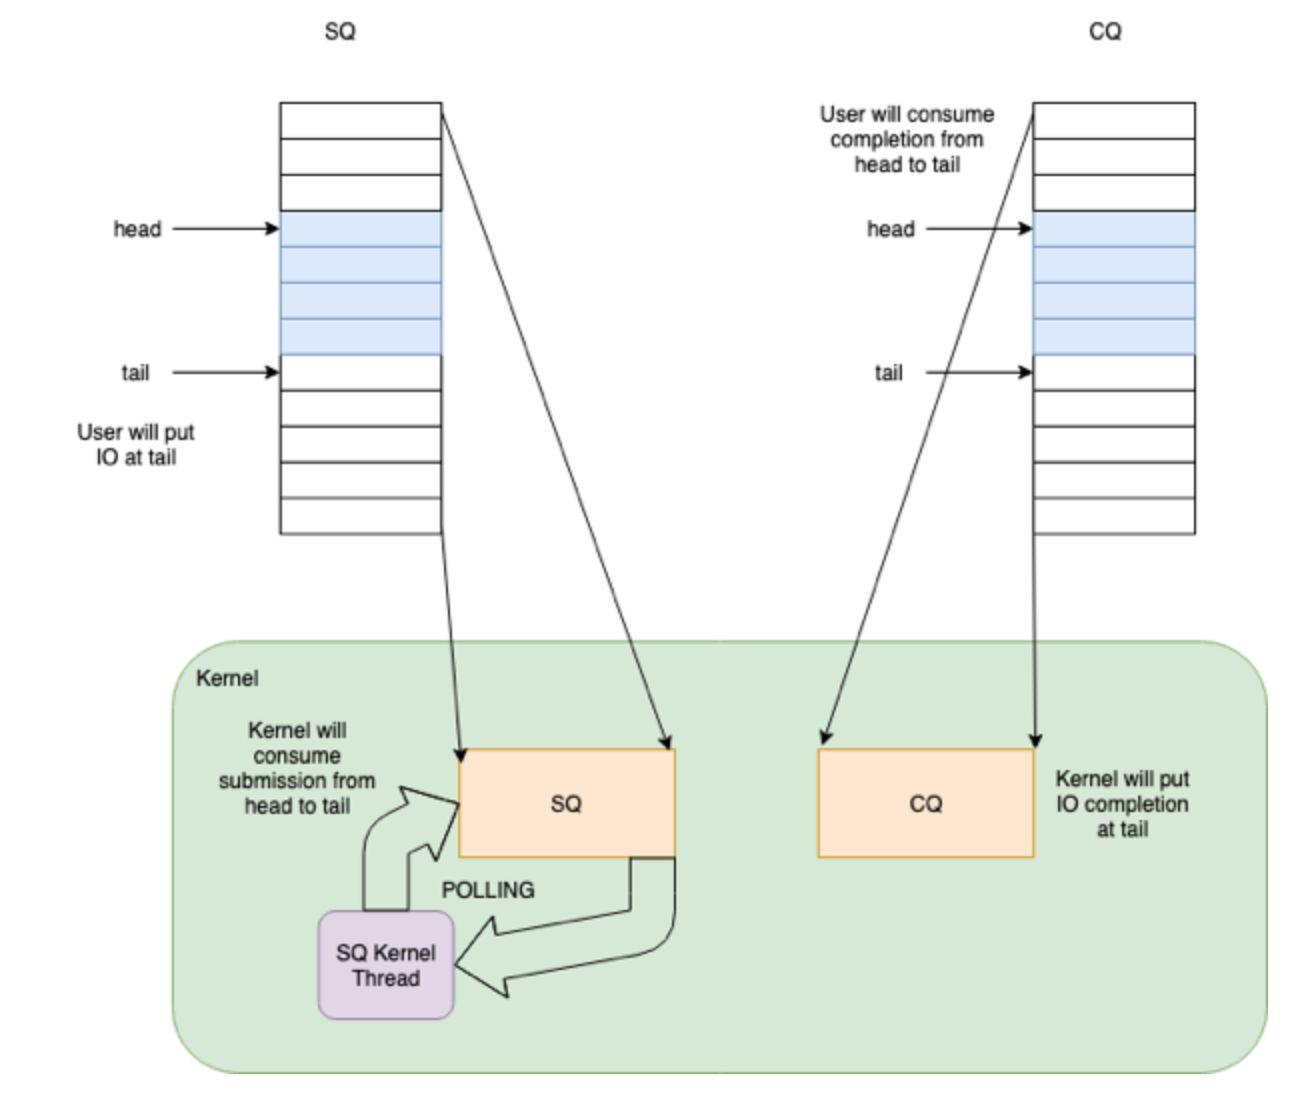
\includegraphics[width=10cm]{images/io_uring.jpg}
    \caption{io\_uring architecture}
    \label{fig:io\_uring architecture}
\end{figure}

\subsubsection{Performances}

Because of the shared ring buffers between the kernel and user space, io\_uring can be a zero-copy system.\\ Copying bytes around becomes necessary when system calls that transfer data between kernel and user space are involved.\\
But since the bulk of the communication in io\_uring is via buffers shared between the kernel and user space, this huge performance overhead is completely avoided.\\ 
While system calls may not seem like a significant overhead, in high performance applications, making a lot of them will begin to matter. \\
So, avoiding system calls as much as possible is a fantastic idea in high-performance applications indeed. \\
While using synchronous programming interfaces or even when using asynchronous programming interfaces under Linux, there is at least one system call involved in the submission of each request.\\
In io\_uring, you can add several requests, simply by adding multiple SQEs each describing the I/O operation you want and make a single call to io\_uring\_enter.


\subsection{Importance for the AOS course}

The project exposes a lot of different concepts treated during the Advanced Operating System course. \\
Allows to dig further into concurrency issues in general and more specifically, event-based concurrency, showing how it is implemented and the different approaches with which it can be treated. \\
Gives the opportunity to learn about different design choices experienced engineers used to develop i/o libraries such as libuv and liburing, showing the trade-off of both of them. \\
To really understand the advantages of one method against the other, a benchmark needs to be implemented. \\
Therefore, a bit of thinking about what metrics to use to evaluate the goodness of a model and the reliability of the outcome obtained is needed.

\subsection{Design and Implementation}

\subsubsection{FSM Server}
At first, the server socket is created using the utility functions in the \textbf{utils.c} file. \\
After the socket has been set, the server is put on an infinite loop, listening for clients connection on port 9090. \\
Once in the loop the server tells the kernel to add a submission queue entry (sqe) in the submission ring. \\
Then the server waits for completion queue entry to become avaiable via the \textbf{io\_uring\_wait\_cqe} call. \\
The program then goes through the list of avaiable cqes, checking for the type of user request, and serving it.
The main method in charge of handling clients requests are the following:

\begin{itemize}
    \item \textbf{add\_accept}: This function, takes the sqe from the submission ring. \\ Using the \textbf{io\_uring\_prep\_accept} sets the sqe with the \textbf{accept} system call, which, used with connection-oriented socket types, it extracts the first connection request on the queue of pending connections for the listening socket fd.
    \item \textbf{add\_socket\_read}: Takes the sqe from the submission ring and sets the sqe with the \textbf{recv} system call, via the \textbf{io\_uring\_prep\_recv} operation. \\ The \textbf{recv} system call is used to read data from a socket.
    \item \textbf{add\_socket\_update}: It updates the state of the client reading the previously received data from the buffer and using the \textbf{compute\_state()} method in the \textbf{state.c} file.\\ It finally sends an ack back to the client with the \textbf{io\_uring\_prep\_send} for benchmarking purposes.
\end{itemize}

In order to improve the performance, the  \textbf{IORING\_FEAT\_FAST\_POLL} has been used. \\
It allows to avoid polling a socket for ready data.  \\
In this way the program can just call a recv (io\_uring\_prep\_recv) on a socket and at the moment there’s data ready it will complete and return as a cqe on your ring.  \\
Because it doesn’t have to poll, it save a system call. \\
Finally, the server has been developed in two different versions, with and without the buffer selection feature. \\

\subsubsection{Buffer Selection}
When applications handle lots of sockets, usually they like to poll for activity on them, then issue IO when they become ready. \\
This approach requires a certain number of system calls, but, at the same time, allows applications to manage how many IO buffers they need. \\
With io\_uring based polled IO, the application need only to issue an \textbf{IORING\_OP\_RECV} (for example, to receive socket data), it doesn't need to poll at all. \\
This means that the application no longer can decide the number of buffers. \\
A possible solution to that comes with the \textbf{IORING\_OP\_PROVIDE\_BUFFERS}. \\
It takes a start address, length of a buffer, and number of buffers. \\
It also provides a group ID with which these buffers should be associated, and a starting buffer ID. \\
The buffers are then added, and the buffer ID is incremented by 1 for each buffer.\\
With that, when doing the same \textbf{IORING\_OP\_RECV}, no buffer is passed in
with the request. \\
When the kernel can satisfy the receive, a buffer is automatically selected from the specified group ID pool. \\
If none are available, the IO is terminated with \textbf{-ENOBUFS}. 


\subsubsection{Benchmark}

In order to evaluate the performances of io\_uring against the other models, a simple benchmarking application has been developed. \\
Using multi-threading, it allows the user to specify the number of TCP clients it wants to create and the period of time (in seconds) it wants them to interact with the server. \\
Each client then repeatedly sends requests to the server for the specified period of time. \\
Each request increments a counter variable, the same applies for the answers made by the server. \\
Once the timer has expired, the overall number of requests and responses are computed, together with the requests/sec and the responses/sec.

\section{Project Outcome}

\subsection{Concrete Outcomes}

The different models have been tested with different number of clients and changing the duration of the test, in order to evaluate the performances. \\
Below, the tables with the results obtained.


\begin{table}[H]
\centering
\begin{tabular}{lllll}
\multicolumn{5}{l}{5 clients, 5 seconds}                         \\
model      & requests & responses & requests/sec & responses/sec \\
select     & 75933    & 75963     & 15186        & 15184         \\
threaded   & 119518   & 119543    & 23903        & 23902         \\
uring\_nbs & 108117   & 108102    & 21623        & 21620         \\
uring\_bs  & 111246   & 111251    & 22249        & 22250         \\
sequential & 51837    & 51837     & 10367        & 10367        
\end{tabular}
\end{table}

\begin{table}[H]
\centering
\begin{tabular}{lllll}
\multicolumn{5}{l}{50 clients, 10 seconds}                       \\
model      & requests & responses & requests/sec & responses/sec \\
select     & 180402   & 180422    & 18040        & 18042         \\
threaded   & 251668   & 251728    & 25166        & 25172         \\
uring\_nbs & 277719   & 277859    & 27771        & 27785         \\
uring\_bs  & 277191   & 277115    & 27719        & 27711         \\
sequential & 100387   & 100388    & 10038        & 10038        
\end{tabular}
\end{table}

\begin{table}[H]
\centering
\begin{tabular}{lllll}
\multicolumn{5}{l}{70 clients, 10 seconds}                       \\
model      & requests & responses & requests/sec & responses/sec \\
select     & 183525   & 183645    & 18352        & 18364         \\
threaded   & 225634   & 225710    & 22563        & 22571         \\
uring\_nbs & 240073   & 240183    & 24007        & 24018         \\
uring\_bs  & 272861   & 272816    & 27286        & 27281         \\
sequential & 128325   & 128325    & 12832        & 12832        
\end{tabular}
\end{table}

The testing has been stopped to 70 clients because after a certain threshold (around 100 clients) the server become unresponsive and crashes. \\
However apart from some inconsistency in the number obtained, the results are good enough to highlight some interesting observation. \\
The main discoveries obtained can be summarized as following:

\begin{itemize}
    \item With a low number of clients, and running the test for a short period of time, the threaded approach wins against the other models. 
    \item The buffer selection approach improve the performances of the model as expected.
    \item After a certain number of clients, the models with io\_uring become the most responsive, outperforming the threaded one.
    \item Sequential model doesn't implement concurrency at all, therefore the performances are obviously the worst.
\end{itemize}

\subsection{Learning Outcomes}

The project allowed me to develop a broader knowledge regarding the different concurrency models. \\
It gave me the opportunity to practice the C programming language, with which i didn't have much experience, working with interesting libraries like liburing and libuv. \\
Finally, developing a simple benchmark, gave me the opportunity to reason about what metrics should be considered when evaluating a model, and showed me that after a certain threshold, stressing the model can results in unexpected behavior.

\subsection{Existing Knowledge}

\begin{itemize}
    \item Advanced Operating Systems (AOS): Concurrency in Linux, event-based concurrency.
    \item Architettura dei Calcolatori e Sistemi Operativi: Basic understanding of Operating Systems.
    \item Fondamenti di Informatica: Basic knowledge of C.
\end{itemize}

\subsection{Problems Encountered}
I have encountered several problems during the development process. \\
Generally speaking the main difficulty has been in trying to understand how liburing could be used. \\
Even though the architecture of io\_uring seems pretty straightforward on paper, the application gave me problems.\\ 
Mainly because working with an asynchronous programming paradigm requires to think about the functioning of the program in an asynchronous manner, which is not something i was used to. \\
Often after having submitted requests in the submission ring i expected to receive the responses from the kernel in the completion ring but i ended up having a different behavior.

\begin{itemize}
    \item In the \textbf{add\_socket\_update} in order to update the state of the client the \textbf{message\_t} struct needs to be filled with the content of the client action, which is then passed in the \textbf{compute\_state} to update the state. \\I had several problems figuring out the correct way to copy the content in the buffer where io\_uring put the data (buf[bid]) in the \textbf{msg.actions} array.\\ I tried several options but i ended up always with segmentation fault. A simple \textbf{memcpy} solved the problem.
    \item The \textbf{state.c} file contains the \textbf{compute\_state} method, which updates the state of the client and print the steps performed.\\ In both the \textbf{uring\_nbs} and \textbf{uring\_bs} files, the action passed to the \textbf{message\_t} was passed as a char value (even though the buf array was an array of \textbf{uint8\_t}). \\However the \textbf{message\_t} struct, defines the actions has an array of \textbf{uint8\_t}.\\ Therefore, when i was passing the action to the       \textbf{compute\_state} method, the \textbf{isValidAction()} always returned false value, given that the action value was translated in a value outside the allowed range (1..4).\\ Therefore i didn't receive any answer when sending requests to the server. \\To solve the issue, i needed to define a char variable having as value the action passed in the \textbf{compute\_state()} method, and passing this variable in the \textbf{isValidAction()} call.
    \item In the benchmark, when using the \textbf{pthread\_create} to instantiate the threads, when using a certain amount of clients, the results computed after the for loop were clearly wrong, with the number of requests and responses being close to 0. \\ I came up with the conclusion that the code for displaying the results, was executed before the threads could correctly finish. \\ Adding a \textbf{sleep()} operation immediately after the for loop solved the issue.
    
\end{itemize}

\section{Honor Pledge}
I pledge that this work was fully and wholly completed within the criteria established for academic integrity by Politecnico di Milano
(Code of Ethics and Conduct) and represents my original production, unless otherwise cited.
I also understand that this project, if successfully graded, will fulfill part B requirement of the Advanced Operating System course
 and that it will be considered valid up until the exam of September 2022.

\begin{flushright}
        Francesco Aristei
\end{flushright}


\end{document}  